% paper/sections/10_3_solver_time.tex
%
% §10.3  ソルバと時間発展の精度検証
%   PPE ソルバ収束特性（欠陥補正法 — 本稿標準），TVD-RK3 時間発展精度
% ═══════════════════════════════════════════════════════════════════════════════
\subsection{ソルバと時間発展の精度検証}
\label{sec:verify_solver}
% ═══════════════════════════════════════════════════════════════════════════════

最後に，圧力 Poisson 方程式（PPE）のソルバと時間積分スキームを検証する．
PPE ソルバは §\ref{sec:verify_spatial} で確認した CCD 演算子を核とする
欠陥補正法であり，等密度ディリクレ（§\ref{sec:verify_ppe}），
Neumann 境界 + ゲージ固定（§\ref{sec:verify_ppe_neumann}），
変密度条件（§\ref{sec:verify_ppe_varrho}；滑らか密度場および界面型密度場）の 3 段階で精度と収束限界を評価する．
時間積分では，CLS 移流用の TVD-RK3（§\ref{sec:verify_tvd_rk3}）と
NS 対流項用の AB2（§\ref{sec:verify_ab2}）の単体精度を ODE テストで検証する．

% ─────────────────────────────────────────────────────────────────────────────
\subsubsection{PPE ソルバ収束特性}
\label{sec:verify_ppe}
% ─────────────────────────────────────────────────────────────────────────────

\noindent\textbf{目的：}
本稿で採用する欠陥補正法（§\ref{sec:defect_correction_main}）が
CCD 演算子の $\Ord{h^6}$ 空間精度を損なわず，少ない反復回数で
発現させることを検証する．
CCD-PPE の直接解法（LU 分解）の詳細は付録~\ref{app:ccd_lu_direct} を参照されたい．

\noindent\textbf{評価対象：}
欠陥補正法の格子収束特性（$k$ 依存性），および FD 直接法との精度・コスト比較．

\noindent\textbf{手順とパラメタ：}
\begin{itemize}[noitemsep]
  \item 2次元 Poisson 方程式，製造解 $p^* = \sin(\pi x)\sin(\pi y)$（$p|_{\partial\Omega}=0$）
  \item $L_H$: CCD 演算子（$\Ord{h^6}$），$L_L$: 2次精度中心差分 FD（\texttt{spsolve}）
  \item 格子 $N = 8, 16, 32, 64, 128$（一様），ディリクレ境界条件
  \item (a) 反復回数 $k = 1, 2, 3, 5, 10$ で打ち切り，$L^\infty$ 誤差と収束次数を計測
  \item (b) 欠陥補正法（$k=3$）vs FD 直接法（$L_L$ のみ）の精度・コスト比較
\end{itemize}
なお，本テストはディリクレ境界条件下で CCD 演算子を用いるため，
§\ref{sec:verify_ccd_convergence} の周期境界テストでは検証されない
CCD 境界スキーム（非周期 BC，$\Ord{h^5}$）の精度検証を兼ねている．

\noindent\textbf{結果：}

\paragraph{(a) 反復回数 $k$ と空間精度の関係．}

\begin{table}[htbp]
\centering
\small
\caption{欠陥補正反復回数 $k$ と空間精度の関係（$L^\infty$ 誤差，$p^* = \sin(\pi x)\sin(\pi y)$）}
\label{tab:dc_iteration_accuracy}
\renewcommand{\arraystretch}{1.3}
\begin{tabular}{ccccccc}
\toprule
$N$ & $h$ & $k=1$ & $k=2$ & $k=3$ & $k=5$ & $k=10$ \\
\midrule
$8$   & $1/8$   & $1.30 \times 10^{-2}$ & $2.71 \times 10^{-4}$ & $2.08 \times 10^{-4}$ & $2.06 \times 10^{-4}$ & $1.98 \times 10^{-4}$ \\
$16$  & $1/16$  & $3.22 \times 10^{-3}$ & $1.13 \times 10^{-5}$ & $1.91 \times 10^{-6}$ & $1.90 \times 10^{-6}$ & $1.81 \times 10^{-6}$ \\
$32$  & $1/32$  & $8.04 \times 10^{-4}$ & $6.54 \times 10^{-7}$ & $1.60 \times 10^{-8}$ & $1.59 \times 10^{-8}$ & $1.53 \times 10^{-8}$ \\
$64$  & $1/64$  & $2.01 \times 10^{-4}$ & $4.04 \times 10^{-8}$ & $1.29 \times 10^{-10}$ & $1.28 \times 10^{-10}$ & $1.23 \times 10^{-10}$ \\
$128$ & $1/128$ & $5.02 \times 10^{-5}$ & $2.52 \times 10^{-9}$ & $1.02 \times 10^{-12}$ & $1.01 \times 10^{-12}$ & $9.77 \times 10^{-13}$ \\
\midrule
\multicolumn{2}{c}{収束次数 $p$} & $\approx 2.0$ & $\approx 4.0$ & $\approx 7.0$ & $\approx 7.0$ & $\approx 7.0$ \\
\bottomrule
\end{tabular}
\end{table}

\begin{figure}[htbp]
\centering
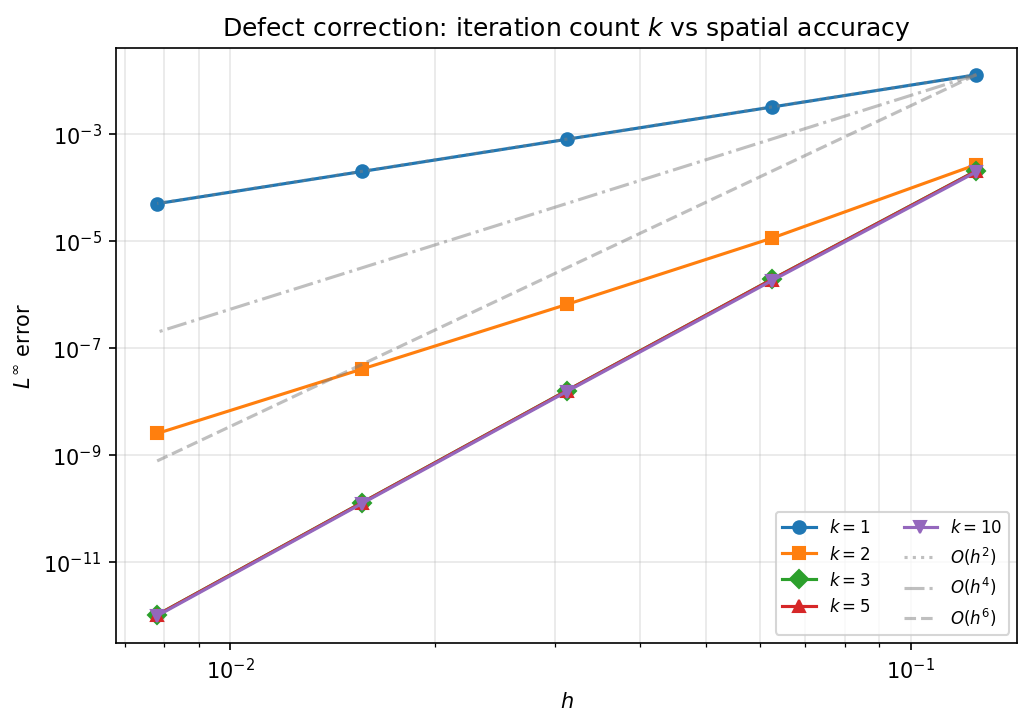
\includegraphics[width=0.72\linewidth]{figures/dc_iteration_convergence}
\caption{欠陥補正反復回数 $k$ と格子収束特性．
$k=1$ では $\Ord{h^2}$（FD 支配），$k=2$ で $\Ord{h^4}$，
$k \geq 3$ で CCD の $\Ord{h^7}$ 精度が発現する．
破線は参照勾配．}
\label{fig:dc_iteration_convergence}
\end{figure}

$k=1$ では $L_L$（$\Ord{h^2}$）が支配的，$k=2$ で $\Ord{h^4}$，
$k \geq 3$ で CCD 精度が完全に発現し $\Ord{h^7}$ に達した．
超収束（$p \approx 7$）はディリクレ解析解が境界上でゼロであるため
境界スキーム（$\Ord{h^5}$）の誤差寄与が消滅することによる．
$k=3$ と $k=10$ で絶対誤差は約 2 倍の差にとどまるため，$k=3$ が実用上の最適値．

\paragraph{(b) 欠陥補正法 vs FD 直接法．}

\begin{table}[htbp]
\centering
\small
\caption{PPE 求解法比較：FD 直接法（$\Ord{h^2}$）vs 欠陥補正法 $k=3$（$\Ord{h^6}$）}
\label{tab:dc_vs_fd}
\renewcommand{\arraystretch}{1.3}
\begin{tabular}{crrcrrcc}
\toprule
$N$ & \multicolumn{2}{c}{FD 直接法} & & \multicolumn{2}{c}{欠陥補正 $k=3$} & 精度比 & コスト比 \\
\cmidrule{2-3} \cmidrule{5-6}
 & $L^\infty$ 誤差 & 次数 & & $L^\infty$ 誤差 & 次数 & & \\
\midrule
$8$   & $1.30 \times 10^{-2}$ & ---  & & $2.08 \times 10^{-4}$ & ---  & $62\times$ & $1.2\times$ \\
$16$  & $3.22 \times 10^{-3}$ & $2.0$ & & $1.91 \times 10^{-6}$ & $6.8$ & $1{,}682\times$ & --- \\
$32$  & $8.04 \times 10^{-4}$ & $2.0$ & & $1.60 \times 10^{-8}$ & $6.9$ & $50{,}219\times$ & --- \\
$64$  & $2.01 \times 10^{-4}$ & $2.0$ & & $1.29 \times 10^{-10}$ & $7.0$ & $1.6 \times 10^{6}$ & $4.0\times$ \\
$128$ & $5.02 \times 10^{-5}$ & $2.0$ & & $1.02 \times 10^{-12}$ & $7.0$ & $4.9 \times 10^{7}$ & $3.4\times$ \\
\bottomrule
\end{tabular}

\smallskip
\noindent 注：コスト比は壁時間の比（欠陥補正 / FD 直接）．
\end{table}

\noindent\textbf{結論：}
欠陥補正法は $k=3$ 回の反復で CCD の $\Ord{h^6}$ 精度を発現させる．
$N=128$ で FD 直接法の $3.4$ 倍のコストで $4{,}900$ 万倍高精度．

% ─────────────────────────────────────────────────────────────────────────────
\subsubsection{TVD-RK3 時間発展精度}
\label{sec:verify_tvd_rk3}
% ─────────────────────────────────────────────────────────────────────────────

\noindent\textbf{目的：}
TVD-RK3（Shu--Osher 3 段 SSP スキーム，§\ref{sec:time_int}）が
設計精度 $\Ord{\Delta t^3}$ を達成することを確認する．

\noindent\textbf{評価対象：}
TVD-RK3 時間積分スキーム（CLS 移流ステップで使用）．

\noindent\textbf{手順とパラメタ：}
ODE $dq/dt = -q$，解析解 $q(T) = e^{-T}$（$T = 1$）．
$n = 16, 32, 64, 128, 256, 512$ ステップで $\Delta t$ を精緻化し，収束次数を計測する．

\noindent\textbf{結果：}

\begin{table}[htbp]
\centering
\caption{TVD-RK3 の ODE 時間精度（$dq/dt = -q$，$T = 1$）}
\label{tab:tvd_rk3_ode}
\renewcommand{\arraystretch}{1.3}
\begin{tabular}{rrrr}
\toprule
ステップ数 $n$ & $\Delta t$ & $|q - e^{-1}|$ & 次数 \\
\midrule
  16 & $6.25 \times 10^{-2}$ & $3.55 \times 10^{-5}$  & ---  \\
  32 & $3.13 \times 10^{-2}$ & $4.39 \times 10^{-6}$  & 3.02 \\
  64 & $1.56 \times 10^{-2}$ & $5.46 \times 10^{-7}$  & 3.01 \\
 128 & $7.81 \times 10^{-3}$ & $6.81 \times 10^{-8}$  & 3.00 \\
 256 & $3.91 \times 10^{-3}$ & $8.51 \times 10^{-9}$  & 3.00 \\
 512 & $1.95 \times 10^{-3}$ & $1.06 \times 10^{-9}$  & 3.00 \\
\bottomrule
\end{tabular}
\end{table}

\noindent\textbf{結論：}
$n \geq 16$ の安定領域で $p \approx 3.00$ の正確な 3 次収束を確認した．

% §10.3.3（旧 10_3a_dc_iteration_accuracy.tex）は上記 paragraph (a) に統合済み．
\label{sec:dc_iteration_accuracy}% backward-compat label

% ─────────────────────────────────────────────────────────────────────────────
\subsubsection{PPE Neumann 境界条件とゲージ固定}
\label{sec:verify_ppe_neumann}
% ─────────────────────────────────────────────────────────────────────────────

\noindent\textbf{目的：}
実際の PPE は全周 Neumann 境界 $\partial p/\partial n = 0$ を課す（§\ref{sec:ppe_bc_stability}）．
Neumann 条件では解が定数分の不定性（零モード）を持つため，
ゲージ固定（1点 $p_{0,0} = p^*(0,0)$ の強制代入）を要する．
本テストでは Neumann BC + ゲージ固定のもとで欠陥補正法の
収束特性を確認し，CCD 境界スキーム（$\Ord{h^5}$）の影響を評価する．

\noindent\textbf{評価対象：}
欠陥補正法（$k=3$），全周 Neumann BC，ゲージ固定 $p_{0,0}=p^*(0,0)$．

\noindent\textbf{手順とパラメタ：}
\begin{itemize}[noitemsep]
  \item 2次元 Poisson 方程式，製造解 $p^* = \cos(\pi x)\cos(\pi y)$
        （$\partial p^*/\partial n = 0$ を自然に満たす）
  \item 格子 $N = 8, 16, 32, 64, 128$（一様），全周 Neumann BC
  \item ゲージ固定：$p_{0,0} = p^*(0,0) = 1$ を強制代入
  \item $L^\infty$ 誤差と収束次数を計測
\end{itemize}

\noindent\textbf{結果：}

\begin{table}[htbp]
\centering
\caption{PPE Neumann BC + ゲージ固定の格子収束（欠陥補正 $k=3$）}
\label{tab:ppe_neumann}
\renewcommand{\arraystretch}{1.3}
\begin{tabular}{rrrr}
\toprule
$N$ & $h$ & $L^\infty$ 誤差 & 次数 \\
\midrule
$8$   & $1/8$   & $1.98 \times 10^{-2}$ & ---  \\
$16$  & $1/16$  & $8.59 \times 10^{-4}$ & $4.5$ \\
$32$  & $1/32$  & $2.87 \times 10^{-5}$ & $4.9$ \\
$64$  & $1/64$  & $9.09 \times 10^{-7}$ & $5.0$ \\
$128$ & $1/128$ & $2.85 \times 10^{-8}$ & $5.0$ \\
\bottomrule
\end{tabular}
\end{table}

\noindent\textbf{結論：}
Neumann BC + ゲージ固定のもとで $p \approx 5.0$ の安定した 5 次収束を確認した．
ディリクレテスト（表~\ref{tab:dc_iteration_accuracy}）の超収束 $\Ord{h^7}$ と異なり，
Neumann BC では解が境界上でゼロとならないため
CCD 境界スキーム（$\Ord{h^5}$）の打ち切り誤差が支配的となり，
$\Ord{h^5}$ に律速される．
これは CCD 内部スキーム（$\Ord{h^6}$）の精度が十分に活かされていることを意味し，
実用上は $\Ord{h^5}$ が全体精度の下限となる．

% ─────────────────────────────────────────────────────────────────────────────
\subsubsection{変密度 PPE の収束特性}
\label{sec:verify_ppe_varrho}
% ─────────────────────────────────────────────────────────────────────────────

\noindent\textbf{目的：}
可変係数演算子 $\bnabla\cdot(1/\rho\,\bnabla p)$（式~\eqref{eq:varrho_product_rule}）を
CCD product-rule 展開（§\ref{sec:ccd_2d_full}）で離散化した場合の収束特性を評価する．
滑らか密度場では $\Ord{h^6}$ 精度の維持を確認し，
界面型密度場（smoothed Heaviside）では一括解法の収束限界を定量的に記録する．

\noindent\textbf{評価対象：}
変密度欠陥補正法（$k=3$）．(a) 滑らか密度場：$\rho_{\max}/\rho_{\min} \approx 1, 9, 99, 999$，
(b) 界面型密度場：$\rho_l/\rho_g = 10, 100, 1000$．

\noindent\textbf{手順とパラメタ：}
\begin{itemize}[noitemsep]
  \item 2次元変密度 Poisson 方程式，製造解 $p^* = \sin(\pi x)\sin(\pi y)$
  \item 滑らか密度場 $\rho(x,y) = 1 + A\sin(\pi x)\cos(\pi y)$，
        $A = 0, 0.8, 0.98, 0.998$
        （$\rho_{\max}/\rho_{\min} \approx 1, 9, 99, 999$）
  \item 右辺 $q = \bnabla\cdot(1/\rho\,\bnabla p^*)$ を解析的に構成
  \item 格子 $N = 16, 32, 64, 128$（一様），ディリクレ BC
  \item 各密度比で $L^\infty$ 誤差・収束次数を計測
\end{itemize}

\noindent\textbf{結果：}

\begin{table}[htbp]
\centering
\small
\caption{変密度 PPE の格子収束（欠陥補正 $k=3$，各密度比）}
\label{tab:ppe_varrho}
\renewcommand{\arraystretch}{1.3}
\begin{tabular}{rcccc}
\toprule
$N$ & $\rho_{\max}/\rho_{\min} = 1$ & $\approx 9$ & $\approx 99$ & $\approx 999$ \\
\midrule
$16$  & $1.91 \times 10^{-6}$ & $2.06 \times 10^{-6}$ & $3.12 \times 10^{-6}$ & $7.79 \times 10^{-6}$ \\
$32$  & $1.60 \times 10^{-8}$ & $1.74 \times 10^{-8}$ & $7.32 \times 10^{-8}$ & $2.67 \times 10^{-7}$ \\
$64$  & $1.29 \times 10^{-10}$ & $1.41 \times 10^{-10}$ & $8.47 \times 10^{-10}$ & $4.76 \times 10^{-9}$ \\
$128$ & $1.02 \times 10^{-12}$ & $1.51 \times 10^{-12}$ & $1.82 \times 10^{-11}$ & $8.50 \times 10^{-11}$ \\
\midrule
次数  & $\approx 7.0$ & $\approx 6.5$ & $\approx 5.5$ & $\approx 5.8$ \\
\bottomrule
\end{tabular}
\end{table}

\noindent\textbf{結論（滑らか密度場）：}
$\rho_{\max}/\rho_{\min} = 1$ では等密度テスト（表~\ref{tab:dc_iteration_accuracy}）の $k=3$ 列と
$L^\infty$ 誤差が一致し，$\Ord{h^{7.0}}$ の超収束を再現した．
密度比 $\approx 9$（$A = 0.8$）でも $\Ord{h^{6.5}}$ が維持される．
$\approx 99$--$999$ では条件数悪化に伴い $\Ord{h^{5.5}}$--$\Ord{h^{5.8}}$ にやや低下するが，
$k = 3$ の固定反復で $N = 128$ 時 $L^\infty = \Ord{10^{-11}}$ と十分な精度を達成した．
ただし，これは密度場が $C^\infty$ 滑らかな場合の結果であり，
実際の二相流で生じる界面型密度場では状況が根本的に異なる．

\paragraph{界面型密度場における収束性の破綻と解決方針（想定内）}
\label{sec:varrho_ppe_limitation}

この破綻は\textbf{想定内}である
（§~\ref{sec:ppe_condition_number} の不連続係数理論から予見される）．
本節ではその発散挙動を定量的に記録し，解決方針を示す．

界面型密度場で製造解テスト（$p^* = \sin\pi x\sin\pi y$，$\rho_l/\rho_g = 10, 100, 1000$）を実施したところ，
欠陥補正法は \textbf{$\rho_l/\rho_g \geq 10$ で発散}した（表~\ref{tab:varrho_interface_divergence}）．
FD 前処理の直接解（DC をスキップ）でも同様に非収束であり，
反復回数 $k$ の増大や緩和係数 $\omega < 1$ の導入によっても収束は得られなかった．

\begin{table}[htbp]
\centering
\caption{界面型密度場での変密度 PPE 収束テスト（DC $k=3$，$N=64$）}
\label{tab:varrho_interface_divergence}
\renewcommand{\arraystretch}{1.2}
\begin{tabular}{rcl}
\toprule
$\rho_l/\rho_g$ & $L^\infty$ 誤差 & 状態 \\
\midrule
$1$    & $1.3 \times 10^{-10}$ & 収束（$\Ord{h^{7.0}}$） \\
$10$   & $1.3$                 & 非収束（振動） \\
$100$  & $1.1 \times 10^{5}$   & 発散 \\
$1000$ & $3.7 \times 10^{3}$   & 発散 \\
\bottomrule
\end{tabular}
\end{table}

\noindent\textbf{原因：}
界面型密度場では $1/\rho$ が界面を挟んで $\rho_l/\rho_g$ 倍のジャンプを持つ．
FD/CCD を問わず，このジャンプを横切るステンシルは $\Ord{1}$ の離散化誤差を生じる．
DC の前処理 $L_L$（FD $\Ord{h^2}$）も同一の問題を抱えるため，
$L_L^{-1}L_H$ のスペクトル半径が 1 を超え，反復が発散する．
これは \textbf{smoothed Heaviside による一括解法の本質的限界}であり，
DC の反復構造や前処理の選択では解消できない．

\noindent\textbf{解決方針：分相 PPE 解法}
各相で定数密度 PPE（$\rho_k^{-1}\nabla^2 p = q$）を独立に解き，
界面上のジャンプ条件 $[p] = \sigma\kappa$ を HFE
（§~\ref{sec:field_extension}）で課すことが考えられる．
これにより不連続係数を横切るステンシルが排除され，
各相の CCD 離散化が $\Ord{h^6}$ の設計精度を回復する．
分相 PPE 解法の実装と検証は今後の主要課題であり，§~\ref{sec:conclusion}で議論する．

% ─────────────────────────────────────────────────────────────────────────────
\subsubsection{AB2 時間積分精度}
\label{sec:verify_ab2}
% ─────────────────────────────────────────────────────────────────────────────

\noindent\textbf{目的：}
NS 方程式の対流項に用いる AB2（Adams--Bashforth 2段，§\ref{sec:ab2_ipc}）が
設計精度 $\Ord{\Delta t^2}$ を達成することを，
TVD-RK3（§\ref{sec:verify_tvd_rk3}）と同一の ODE テストで確認する．

\noindent\textbf{評価対象：}
AB2 時間積分スキーム（NS 対流項専用，初回ステップは前進 Euler）．

\noindent\textbf{手順とパラメタ：}
ODE $dq/dt = -q$，解析解 $q(T) = e^{-T}$（$T = 1$）．
$n = 16, 32, 64, 128, 256, 512$ ステップで $\Delta t$ を精緻化し，収束次数を計測する．
$n=0$ は前進 Euler（§\ref{sec:ab2_ipc}，注意~\ref{warn:ab2_startup}），
$n \ge 1$ で AB2 に切り替える．

\noindent\textbf{結果：}

\begin{table}[htbp]
\centering
\caption{AB2 の ODE 時間精度（$dq/dt = -q$，$T = 1$，初回 Euler）}
\label{tab:ab2_ode}
\renewcommand{\arraystretch}{1.3}
\begin{tabular}{rrrr}
\toprule
ステップ数 $n$ & $\Delta t$ & $|q - e^{-1}|$ & 次数 \\
\midrule
  16 & $6.25 \times 10^{-2}$ & $1.42 \times 10^{-4}$  & ---  \\
  32 & $3.13 \times 10^{-2}$ & $3.27 \times 10^{-5}$  & 2.12 \\
  64 & $1.56 \times 10^{-2}$ & $7.84 \times 10^{-6}$  & 2.06 \\
 128 & $7.81 \times 10^{-3}$ & $1.92 \times 10^{-6}$  & 2.03 \\
 256 & $3.91 \times 10^{-3}$ & $4.73 \times 10^{-7}$  & 2.02 \\
 512 & $1.95 \times 10^{-3}$ & $1.18 \times 10^{-7}$  & 2.01 \\
\bottomrule
\end{tabular}
\end{table}

\noindent\textbf{結論：}
$n \geq 16$ で $p \approx 2.0$ の正確な 2 次収束を確認した．
初回 Euler ステップ（$n=0$）の $\Ord{\Delta t}$ 寄与は寄生根減衰（$|\rho_2|=0.5$）により
数ステップで無視できるレベルに減衰し，全体精度 $\Ord{\Delta t^2}$ に影響しない
（§\ref{sec:ab2_ipc} 参照）．
